%==============================================================================
% USF — Unit-Streamed Fine-Tuning. Paper 1 (the streaming system).
% Elsevier elsarticle format, for submission to High-Confidence Computing.
% Derived from main.tex (IEEEtran) -- content is identical; only the
% document-class-specific scaffolding (front matter, proof environments,
% bibliography style) changed to match elsarticle's conventions.
% RULE: every number in this paper is measured. No placeholders.
%==============================================================================
\documentclass[preprint,12pt]{elsarticle}

\usepackage[T1]{fontenc}
\usepackage[utf8]{inputenc}
\usepackage{graphicx}
\usepackage{booktabs}
\usepackage{amsmath,amssymb,amsthm}
\usepackage{mathtools}
\usepackage{algorithm}
\usepackage{algpseudocode}
\usepackage{enumitem}
\usepackage{xcolor}
\usepackage{tikz}
\usetikzlibrary{arrows.meta}
\usepackage[hidelinks]{hyperref}
\usepackage{cleveref}

% Fig. 1 palette: a visit either pays a disk read or finds the unit resident.
\definecolor{ioload}{RGB}{178,24,43}
\definecolor{iohit}{RGB}{33,102,172}

\newtheorem{theorem}{Theorem}
\newtheorem{corollary}[theorem]{Corollary}
\newtheorem{proposition}[theorem]{Proposition}
\newtheorem{definition}[theorem]{Definition}
\newtheorem{remark}[theorem]{Remark}

\crefname{figure}{Fig.}{Figs.}
\Crefname{figure}{Fig.}{Figs.}

\newcommand{\usf}{USF}
\newcommand{\VJP}{\mathrm{VJP}}
\newcommand{\Wu}{\lvert W_u \rvert}
\newcommand{\sthree}{S\textsuperscript{3}}

\journal{High-Confidence Computing}

\begin{document}

\begin{frontmatter}

\title{\usf{}: Unit-Streamed Fine-Tuning of Large Language Models with Exact Gradients on
Consumer GPUs\tnoteref{t1}}
\tnotetext[t1]{Manuscript prepared July 2026. All experiments were carried out on a single
laptop-class NVIDIA GeForce GTX~1050 (Mobile, 3.94\,GB, no tensor cores).}

\author[utp]{Nicolas Andrey Orozco Giraldo\corref{cor1}\fnref{orcid1}}
\ead{nicolas.orozco@utp.edu.co}
\author[utp]{Luis Eduardo Muñoz Guerrero\fnref{orcid2}}
\ead{lemunozg@utp.edu.co}
\author[udea]{Yony Fernando Ceballos\fnref{orcid3}}
\ead{yony.ceballos@udea.edu.co}

\cortext[cor1]{Corresponding author}
\fntext[orcid1]{ORCID: \url{https://orcid.org/0000-0002-6332-9757}}
\fntext[orcid2]{ORCID: \url{https://orcid.org/0000-0002-9414-6187}}
\fntext[orcid3]{ORCID: \url{https://orcid.org/0000-0001-5787-8832}}

\address[utp]{Universidad Tecnológica de Pereira, Pereira, Colombia}
\address[udea]{Facultad de Ingeniería, Grupo de Ingeniería y Sociedad, Universidad de Antioquia,
Medellín, Colombia}

\begin{abstract}
Fine-tuning a 7B-parameter language model conventionally requires 8--16\,GB of GPU memory, because
the frozen base must remain resident throughout the forward and backward passes. That requirement
is what excludes anyone without data-centre-class hardware from fine-tuning models at this scale at
all, regardless of how few parameters they intend to train. We show that the requirement comes from
implementation choices, not from mathematical necessity. Reverse-mode
differentiation composes \emph{local} vector--Jacobian products: the gradient at layer $i$ depends
only on that layer's input, its weights, and the incoming cotangent, never on the other $L-1$
layers. We introduce \emph{Unit-Streamed Fine-Tuning} (\usf), which keeps exactly one weight unit
resident at a time, streamed from disk, and prove that the resulting gradients are \emph{exact}
(Theorem~\ref{thm:exact}) and not approximate. The consequence is a memory bound independent of model
depth and of total parameter count: only the largest single unit matters (Theorem~\ref{thm:vram}). We
further prove that inverting the loop order (\emph{layer-major}, Theorem~\ref{thm:lm}) divides disk
traffic by the gradient-accumulation factor $G$ while leaving gradients bit-identical, moving the
system from I/O-bound to compute-bound. On a laptop-class GTX~1050 (3.94\,GB, no tensor cores)---a
deliberately unfavourable choice, since a bound that holds here holds on essentially any GPU a
practitioner might own---we fine-tune Qwen2.5-7B (15.2\,GB
of weights on disk) at an allocator peak of 2.2\,GB, or 2.9\,GB of total device occupancy
including the CUDA context, reducing held-out perplexity from 9.52 to 4.46. Layer-major is verified gradient-exact
on the 7B model itself ($\max|\Delta|=0$ over 1400 tensors) and yields a measured $1.40\times$
speed-up, and a predictive cost model matches measurements within 6\%. \usf{} is adapter-agnostic: a
spectral adapter and LoRA both run unmodified. Under the same budget, 4-bit quantization does not
fit (5.43\,GB required). The bound predicts that Llama-3-70B fits the same card at the implemented
granularity.
\end{abstract}

\begin{keyword}
Parameter-efficient fine-tuning \sep memory-constrained training \sep large language models \sep
exact gradients \sep out-of-core computation \sep automatic differentiation \sep consumer hardware
\end{keyword}

\end{frontmatter}

%==============================================================================
\section{Introduction}
\label{sec:intro}

Parameter-efficient fine-tuning (PEFT) reduced the \emph{trainable} footprint of
adapting large language models by orders of magnitude: LoRA~\cite{hu2022lora} updates well under
$1\%$ of the weights, and adapters~\cite{houlsby2019adapters} or prompt
tuning~\cite{lester2021prompt} update fewer still. The \emph{resident} footprint, however, did not
follow. Whatever the adapter, the frozen base must be present during both the forward and the
backward pass, so adapting a 7B model in half precision still demands 8--16\,GB of device memory.
The practical effect is a hardware census: researchers whose GPU holds 4\,GB are excluded from
working with 7B models at all, irrespective of how few parameters they intend to train.

Quantization attacks the constant~\cite{dettmers2023qlora,dettmers2022int8}, compressing the
resident base by a factor of four to eight. It does not attack the coupling. A 4-bit 7B model
still occupies several gigabytes, a 4-bit 70B model still exceeds any consumer card, and the
compression is paid for in accuracy. Offloading frameworks such as
ZeRO-Infinity~\cite{rajbhandari2021zeroinfinity} do move parameters off the device, but they were
designed for a different setting: training \emph{all} weights across a cluster, where the dominant
problem is sharding optimizer state.

\subsection{The observation}

This paper begins from an elementary property of reverse-mode differentiation
\cite{griewank2008evaluating,baydin2018autodiff} that, to our knowledge, has not been exploited to
its logical conclusion in this setting. Backpropagation is a composition of \emph{local}
vector--Jacobian products (VJPs). To differentiate through layer $i$ one requires that layer's
input, that layer's weights, and the incoming cotangent, and nothing else. The remaining $L-1$
layers are irrelevant \emph{at that instant}. Keeping the whole model resident is therefore a
choice made for speed, not a requirement imposed by correctness.

We take that observation literally. \usf{} holds exactly one weight \emph{unit} in device memory at
a time, streams it from disk, computes, releases it, and re-streams it during the backward pass.
The immediate question is whether this costs accuracy. It does not: we prove
(Theorem~\ref{thm:exact}) and verify ($\max|\Delta|=0$) that the gradients are identical to those of
ordinary full-graph autograd. \usf{} is not an approximation.

\subsection{The consequence}

Once residency is decoupled from correctness, the memory bound changes shape. The peak is set by
the largest \emph{single} unit:
\begin{equation}
\label{eq:headline}
\mathrm{VRAM}_{\text{peak}} \;\approx\; \max_u \Wu \cdot s \;+\; |\theta|\cdot s_{\text{opt}} \;+\; A ,
\end{equation}
which depends neither on the depth $L$ nor on the total size $\sum_i |W_i|$
(Theorem~\ref{thm:vram} and its corollaries). Adding layers to a model does not increase its memory
requirement; it increases only time and disk traffic. Model size ceases to be a memory problem and
becomes a storage-and-time problem. It is this decoupling, and not any single engineering
component, that we regard as the contribution of this work.

A second result follows from the same locality. Because gradient accumulation is a sum, and sums
are order-invariant, the two nested loops of a training step (over micro-batches and over
layers) may be exchanged. Keeping a unit resident while all $G$ micro-batches pass through it
divides disk traffic by $G$ with bit-identical gradients (Theorem~\ref{thm:lm}). This reordering is
pointless when the model fits in memory, which is presumably why the literature does not consider
it; under streaming it is the dominant optimization, and it moves the system from I/O-bound to
compute-bound.

\subsection{Contributions}

\begin{enumerate}[leftmargin=*, label=\arabic*)]
\item \textbf{A size-independence result.} We prove that the memory required to fine-tune a frozen
model is a function of its largest streamable unit alone, independent of depth and of total
parameter count (Theorem~\ref{thm:vram}, Corollary~\ref{cor:depth}, Corollary~\ref{cor:size}).
\item \textbf{Exactness, proved and verified.} \usf{} preserves gradients exactly
(Theorem~\ref{thm:exact}); we measure $\max|\Delta|=0$, including on the 7B model itself
(Section~\ref{sec:exp}).
\item \textbf{Layer-major streaming.} Exchanging the loop order divides I/O by the accumulation
factor $G$ at no cost in correctness (Theorem~\ref{thm:lm}), changing the performance regime
(Section~\ref{sec:cost}).
\item \textbf{A predictive cost model} that matches measurement within 6\% (Section~\ref{sec:cost}),
which is why we treat the scaling statements in Section~\ref{sec:scaling} as predictions rather than
extrapolations.
\item \textbf{An adapter- and model-agnostic system.} The same infrastructure runs LoRA and a
spectral adapter unmodified (Corollary~\ref{cor:agnostic}), and selects its streaming granularity
automatically from the available memory (Section~\ref{sec:auto}).
\end{enumerate}

We \emph{demonstrate} 7B on a 4\,GB card; we \emph{predict}, from a
proved bound and a validated cost model, that 70B fits the same card with the machinery we
implement; and we identify precisely which unimplemented extension a 405B model would require
(Section~\ref{sec:scaling}). We do not claim the latter two as results.

%==============================================================================
\section{Related Work}
\label{sec:related}

\textbf{Parameter-efficient fine-tuning.} LoRA~\cite{hu2022lora} and its
descendants~\cite{liu2024dora}, adapters~\cite{houlsby2019adapters}, and prompt
tuning~\cite{lester2021prompt} minimise \emph{trainable} parameters. They are orthogonal to this
work: \usf{} governs where computation lives, not what is adapted, and
Corollary~\ref{cor:agnostic} makes this formal. We evaluate LoRA and a spectral adapter under \usf{} without
modifying either.

\textbf{Quantization.} QLoRA~\cite{dettmers2023qlora} and LLM.int8()~\cite{dettmers2022int8}
shrink the resident base by compressing it. The axis is different from ours in two respects.
First, quantization buys memory with \emph{accuracy}, whereas \usf{} buys it with \emph{time} and
is exact (Corollary~\ref{cor:noapprox}). Second, it improves the constant but preserves the coupling to
model size; Section~\ref{sec:quant} reports the concrete consequence, namely that 4-bit is infeasible on
our budget while \usf{} is not. The two are composable, and we do not present them as
alternatives.

\textbf{Offloading and sharding.} ZeRO~\cite{rajbhandari2020zero},
ZeRO-Offload~\cite{ren2021zerooffload} and ZeRO-Infinity~\cite{rajbhandari2021zeroinfinity}
established that parameters and optimizer state can reside off-device, and are the closest prior
art. The regime differs on the point that matters. Those systems target training in which every
weight is trainable, distributed over a cluster; their central difficulty, and their main
contribution, is partitioning optimizer state, whose size is proportional to the trainable
parameter count. In our regime $|\theta| \ll |W|$, so there is no optimizer state worth
partitioning, and the problem collapses entirely onto the residency of $W$. What we add is
therefore not offloading per se, but (i) the formal bound and its independence of model size
(Theorem~\ref{thm:vram}), (ii) the granularity hierarchy that determines feasibility
(Theorem~\ref{thm:gran}), and (iii) the layer-major reordering (Theorem~\ref{thm:lm}), which has no purpose in a
regime where the model is resident. Production dispatch libraries such as
\texttt{accelerate}~\cite{accelerate2022} provide module-level CPU/disk placement aimed principally
at inference; Section~\ref{sec:quant} reports our measurements with that path.

\textbf{Recomputation.} Activation checkpointing~\cite{chen2016checkpointing} and the classical
\textsc{Revolve} schedules~\cite{griewank2000revolve} trade compute for memory by discarding and
recomputing \emph{activations}. This is orthogonal and complementary: we use checkpointing, and
additionally discard and re-stream the \emph{weights}. To our knowledge the storage/recomputation
trade-off has not previously been applied to frozen weights with an accompanying exactness
guarantee.

\textbf{I/O-aware design.} FlashAttention~\cite{dao2022flashattention} demonstrated that
reorganising a computation around its memory traffic, without altering its result, yields
substantial gains, and that exactness need not be sacrificed for speed. \usf{} shares
that philosophy at a different level of the hierarchy: FlashAttention minimises traffic between
on-chip and high-bandwidth memory within attention, whereas \usf{} governs traffic between disk and
device for the weights of the entire model. Theorem~\ref{thm:lm} is an I/O-aware scheduling result in the
same spirit, and Section~\ref{sec:cost} follows the roofline reasoning of~\cite{williams2009roofline} in
identifying which resource binds.

\textbf{Pipelining.} GPipe~\cite{huang2019gpipe} and related
approaches~\cite{jia2019beyond} partition layers across devices and overlap micro-batches to fill
the pipeline. Superficially, layer-major (Theorem~\ref{thm:lm}) resembles a pipeline schedule; the purpose
is inverted. Pipelining distributes a model too large for one device across many; layer-major keeps
one device and amortises the cost of \emph{re-reading} the model, an expense that only exists when
weights are streamed.

%==============================================================================
\section{Preliminaries}
\label{sec:prelim}

Let a frozen transformer of $L$ layers compute $h_0 = E(x)$,
$h_i = f_i(h_{i-1}; W_i, \theta_i)$ for $i=1,\dots,L$, and $\ell = C(h_L,y)$, where $W_i$ are the
\emph{frozen} weights of layer $i$ and $\theta_i$ the \emph{trainable} adapter parameters. Because
the base is frozen, $\nabla_{W_i}\ell$ is never required---only $\nabla_{\theta}\ell$. We assume
the PEFT regime $|\theta| \ll |W|$ throughout, and we write $s$ for bytes per scalar ($s=2$ in
fp16), $B$ for micro-batch size, $S$ for sequence length, $d$ for model width, and $G$ for the
number of gradient-accumulation steps.

\begin{definition}[Streamable unit]
\label{def:unit}
A \emph{unit} $u$ is a subset of weights that can be loaded and released independently, and
$\mathcal{U}$ denotes a partition of $\{W_i\}$ into such units. We consider three nested
granularities: \emph{layer} (an entire decoder block), \emph{sublayer} (the attention block and
the MLP block separately), and \emph{matrix} (a single projection).
\end{definition}

\begin{definition}[Streaming operators]
\label{def:ops}
$\textsc{Load}(u)$ materialises $W_u$ from disk into device memory at an I/O cost of $\Wu$ bytes;
$\textsc{Free}(u)$ returns $W_u$ to a placeholder device, releasing the memory at no I/O cost. The
two are strictly nested: no other unit is loaded between a $\textsc{Load}(u)$ and its matching
$\textsc{Free}(u)$.
\end{definition}

Algorithm~\ref{alg:usf} states the base algorithm. The forward pass builds no autograd graph: activations
\emph{and} weights are discarded, and each layer is recomputed, with its weights re-streamed,
during the backward pass.

\begin{algorithm}[t]
\caption{\usf{} (batch-major, layer granularity)}
\label{alg:usf}
\begin{algorithmic}[1]
\State $h \gets E(x)$
\For{$i = 1$ \textbf{to} $L$} \Comment{forward, no graph}
    \State $c_i \gets h$ \Comment{checkpoint: input of layer $i$}
    \State $\textsc{Load}(W_i)$; \; $h \gets f_i(h; W_i, \theta_i)$; \; $\textsc{Free}(W_i)$
\EndFor
\State $\ell \gets C(h,y)$; \; $g \gets \partial\ell/\partial h_L$
\For{$i = L$ \textbf{down to} $1$} \Comment{backward, re-streaming}
    \State $x \gets c_i$ with gradient tracking enabled
    \State $\textsc{Load}(W_i)$
    \State $\hat h \gets f_i(x; W_i, \theta_i)$ \Comment{recompute \emph{with} graph}
    \State $\hat h.\textsc{Backward}(g)$ \Comment{accumulate $\partial\ell/\partial\theta_i$}
    \State $\textsc{Free}(W_i)$; \; $g \gets x.\mathrm{grad}$
\EndFor
\end{algorithmic}
\end{algorithm}

%==============================================================================
\section{Exactness}
\label{sec:exact}

The defining property of \usf{} is that streaming is not an approximation. This separates it
categorically from quantization, which trades memory for accuracy.

\begin{theorem}[Gradient exactness]
\label{thm:exact}
Let $\nabla_\theta \ell^{\mathrm{full}}$ be the gradient produced by reverse-mode differentiation
over the complete computational graph with every $W_i$ resident, and let
$\nabla_\theta \ell^{\usf}$ be the gradient produced by Algorithm~\ref{alg:usf}. Then, in exact arithmetic,
\begin{equation}
\nabla_\theta \ell^{\usf} \;=\; \nabla_\theta \ell^{\mathrm{full}} .
\end{equation}
\end{theorem}

\begin{proof}
Reverse-mode differentiation computes, for each layer $i$, the pair
\begin{equation}
\label{eq:vjp}
\left(\frac{\partial\ell}{\partial\theta_i},\; \frac{\partial\ell}{\partial h_{i-1}}\right)
= \VJP_{f_i}\!\left(h_{i-1}, W_i, \theta_i;\; \frac{\partial\ell}{\partial h_i}\right).
\end{equation}
The map in~\eqref{eq:vjp} is \emph{local}: it is a function of (a) the evaluation point $h_{i-1}$,
(b) the parameters $W_i,\theta_i$, and (c) the incoming cotangent $\partial\ell/\partial h_i$
alone. It does not depend on $W_j$ for any $j \neq i$.

Algorithm~\ref{alg:usf} supplies all three unchanged. For (a), the checkpoint $c_i = h_{i-1}$ is recorded
during the forward pass, so the recomputation is evaluated at the identical point, with no
approximation. For (b), $\textsc{Load}(W_i)$ restores $W_i$ bit-for-bit, since it re-reads the same
tensor from disk, while $\theta_i$ is resident and unmodified within a step. For (c),
$g=\partial\ell/\partial h_i$ holds by backward induction from $g_L = \partial\ell/\partial h_L$.

Every local VJP is therefore evaluated at exactly the point at which it would be evaluated in the
full graph, and their composition, which is exactly the chain rule, yields the same value.
Finally, $\textsc{Free}(W_i)$ only relocates a tensor: arithmetic is invariant to device placement.
\end{proof}

\begin{corollary}[Not an approximation]
\label{cor:noapprox}
\usf{} introduces no error, bias, or variance. Any deviation from the full-graph gradient is
confined to the ordinary non-determinism of floating-point arithmetic (Remark~\ref{rem:fp}).
\end{corollary}

\begin{corollary}[Adapter agnosticism]
\label{cor:agnostic}
Theorem~\ref{thm:exact} uses no property of $f_i$ beyond differentiability. \usf{} is therefore
independent of the adapter: it applies verbatim to LoRA, to spectral adapters, or to any
parameterisation of $\theta$. We verify this with two different adapters in Section~\ref{sec:exp}.
\end{corollary}

\begin{remark}[Floating-point considerations]
\label{rem:fp}
Theorem~\ref{thm:exact} asserts equality in exact arithmetic; two points deserve care in practice. First,
weights are preserved exactly: $\textsc{Load}$ re-reads the same fp16 tensor, so no requantisation
occurs, and this holds unconditionally. Second, if the recomputation selects a different kernel
from the original forward, floating-point reduction order may differ in the last bits. This is the
non-determinism inherent to standard activation checkpointing~\cite{chen2016checkpointing} and is
not specific to \usf{}. In our measurements, with identical shapes and kernels, agreement is exact
(Table~\ref{tab:exact}).
\end{remark}

%==============================================================================
\section{The Memory Bound}
\label{sec:vram}

\begin{theorem}[Peak memory]
\label{thm:vram}
Under Algorithm~\ref{alg:usf} with granularity $\mathcal{U}$, the peak device memory satisfies
\begin{equation}
\label{eq:vram}
\mathrm{VRAM}_{\text{peak}} \le \underbrace{\max_u \Wu \cdot s}_{\text{resident unit}}
+ \underbrace{|\theta|\cdot s_{\text{opt}}}_{\text{adapters}}
+ \underbrace{A}_{\text{activations}}
+ \underbrace{K}_{\text{checkpoints}},
\end{equation}
where $A$ is the internal activation memory of a \emph{single} unit and
$K = L\cdot B\cdot S\cdot d\cdot s$ if the checkpoints $\{c_i\}$ reside on device.
\end{theorem}

\begin{proof}
At every instant of Algorithm~\ref{alg:usf} exactly one unit is loaded, since $\textsc{Load}$ and
$\textsc{Free}$ are strictly nested and non-overlapping (Definition~\ref{def:ops}); this yields the first
term. The adapters are resident by construction: $\theta$ is updated every step and its optimizer
state must persist across steps; its size is $|\theta| \ll |W|$ by the PEFT hypothesis. A
gradient-carrying graph exists only within the iteration of one unit, because the forward pass
builds no graph; this yields $A$. Finally, the $c_i$ are the only tensors that survive between
iterations.
\end{proof}

\begin{corollary}[Independence of depth]
\label{cor:depth}
The checkpoints $c_i$ are activations, and unlike weights they are not required on device between
their production and their use. Offloading them to host memory gives $K \approx 0$ and hence
\begin{equation}
\mathrm{VRAM}_{\text{peak}} \;\approx\; \max_u \Wu \cdot s + |\theta| \cdot s_{\text{opt}} + A ,
\end{equation}
which is independent of $L$. Adding layers to a model does not increase its memory requirement.
\end{corollary}

\begin{corollary}[Independence of model size]
\label{cor:size}
The bound does not contain $\sum_i |W_i|$. Two models whose largest unit has the same size have
the same memory requirement, however different their total parameter counts.
\end{corollary}

Corollary~\ref{cor:size} is the paper's central claim. It does not say that a larger model is as cheap to
fine-tune as a smaller one: the I/O and
compute costs both scale with $\sum_i |W_i|$, as Section~\ref{sec:cost} quantifies. It says that those
costs are paid in \emph{time}, not in \emph{memory}. The device requirement is set by the largest
single unit and by nothing else, which is why the granularity hierarchy of the next section
determines feasibility.

%==============================================================================
\section{Granularity}
\label{sec:gran}

\begin{theorem}[Granularity hierarchy]
\label{thm:gran}
For the nested partitions of Definition~\ref{def:unit},
\begin{equation}
\max_{i,p} |W_{i,p}| \;\le\; \max_i \max\!\left(|W_i^{\text{attn}}|, |W_i^{\text{mlp}}|\right)
\;\le\; \max_i |W_i| ,
\end{equation}
and Theorem~\ref{thm:vram} applies to any of them. Refining the granularity reduces peak memory
monotonically at identical total I/O.
\end{theorem}

\begin{proof}
The partitions are nested (matrix $\subset$ sublayer $\subset$ layer), and a maximum over a finer
partition cannot exceed the maximum over a coarser one. The total I/O per pass is
$\sum_u \Wu = \sum_i |W_i|$, which is invariant to the partition: the same bytes are read, in
smaller pieces.
\end{proof}

Table~\ref{tab:scaling} instantiates Theorem~\ref{thm:gran} for four model families. Two observations follow.
Llama-3-70B~\cite{grattafiori2024llama3} fits a 3.94\,GB card at \emph{layer} granularity, with
1.59\,GB per block; no refinement is needed. A 405B model does not fit at layer or sublayer
granularity, but its largest single matrix occupies 1.62\,GB and would fit: this is Corollary~\ref{cor:size}
taken to its extreme.

\begin{remark}[Implementation limit]
\label{rem:matrixlimit}
Theorem~\ref{thm:gran} is a statement about partitions and holds at matrix granularity. Our
\emph{implementation}, however, supports layer and sublayer granularity only. The reason is
an engineering limitation, not a mathematical one: we delegate attention to the reference
implementation~\cite{wolf2020transformers}, which consumes $W_q, W_k, W_v, W_o$ jointly within a
single call. Streaming them individually would require reimplementing the attention internals,
including rotary embeddings~\cite{su2024roformer} and grouped-query
attention~\cite{shazeer2019mqa}, a substitution we judged to carry more risk of silent
incorrectness than the benefit warrants. We therefore claim 70B by the bound at an implemented
granularity, and we claim nothing for 405B beyond Table~\ref{tab:scaling}.
\end{remark}

\begin{table}[t]
\centering
\caption{Unit size by granularity (fp16). The adapters, activations and checkpoints add under
0.6\,GB. Values are computed from the published architecture configurations by the same code that
drives the streamer.}
\label{tab:scaling}
\footnotesize
\setlength{\tabcolsep}{4pt}
\begin{tabular}{@{}lrrrrc@{}}
\toprule
\textbf{Model} & $L$ & \textbf{layer} & \textbf{attn/mlp} & \textbf{matrix} & \textbf{4\,GB?} \\
\midrule
Qwen2.5-7B    & 28  & 0.43\,GB & 0.05 / 0.38 & 0.13\,GB & any granularity \\
Llama-3-8B    & 32  & 0.41\,GB & 0.08 / 0.33 & 0.11\,GB & any granularity \\
13B-class     & 40  & 0.59\,GB & 0.20 / 0.40 & 0.13\,GB & any granularity \\
Llama-3-70B   & 80  & 1.59\,GB & 0.28 / 1.31 & 0.44\,GB & \textbf{layer} \\
Llama-3-405B  & 126 & 5.94\,GB & 1.06 / 4.88 & \textbf{1.62\,GB} & matrix only$^\dagger$ \\
\bottomrule
\end{tabular}
\\[2pt]
\raggedright\footnotesize $^\dagger$ Matrix granularity is not implemented; see
Remark~\ref{rem:matrixlimit}.
\end{table}

%==============================================================================
\section{Layer-Major Streaming}
\label{sec:lm}

Algorithm~\ref{alg:usf} is \emph{batch-major}: for each micro-batch it traverses all $L$ units. With
accumulation over $G$ micro-batches, the model is therefore read $G$ times per optimizer step. The
following reordering removes that factor.

\begin{definition}[Layer-major]
\label{def:lm}
Exchange the two loops: hold unit $u$ resident and pass all $G$ micro-batches through it before
advancing to $u+1$. The backward pass is symmetric: one load of $W_i$, then $G$ local
backpropagations.
\end{definition}

Figure~\ref{fig:schedule} shows why this matters. The two schedules visit exactly the same set of
(unit, micro-batch) pairs, and by Theorem~\ref{thm:exact} each visit computes the same local VJP; they
differ only in the order of the traversal, and therefore in how many of those visits find the unit
already resident.

\begin{figure}[t]
\centering
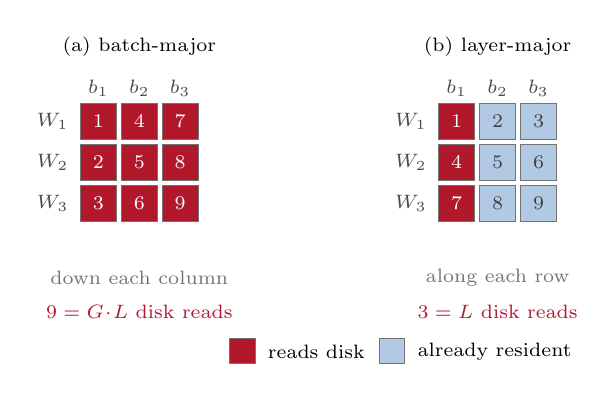
\begin{tikzpicture}[
  cell/.style={draw=black!55, line width=0.3pt, minimum size=4.6mm, inner sep=0,
               font=\scriptsize, text=white},
  load/.style={cell, fill=ioload},
  hit/.style={cell, fill=iohit!35, text=black!75},
  hdr/.style={font=\scriptsize\itshape, text=black!70},
  note/.style={font=\scriptsize},
]
\foreach \panel/\xo in {a/0, b/4.55} {
  % column headers: micro-batches
  \foreach \j in {1,2,3} {
    \node[hdr] at (\xo+\j*0.52, 0.42) {$b_\j$};
  }
  % row headers: units
  \foreach \i in {1,2,3} {
    \node[hdr] at (\xo-0.06, -\i*0.52+0.52) {$W_\i$};
  }
}
% ---- (a) batch-major: every visit pays a disk read -> G*L loads
\foreach \i in {1,2,3} {
  \foreach \j in {1,2,3} {
    \pgfmathtruncatemacro{\ord}{(\j-1)*3+\i}
    \node[load] at (\j*0.52, -\i*0.52+0.52) {\ord};
  }
}
% ---- (b) layer-major: only the first visit of each row pays
\foreach \i in {1,2,3} {
  \foreach \j in {1,2,3} {
    \pgfmathtruncatemacro{\ord}{(\i-1)*3+\j}
    \ifnum\j=1
      \node[load] at (4.55+\j*0.52, -\i*0.52+0.52) {\ord};
    \else
      \node[hit] at (4.55+\j*0.52, -\i*0.52+0.52) {\ord};
    \fi
  }
}
% Traversal order: the cell numbers already carry it; these only name the pattern.
\node[note, text=black!55] at (1.04,-1.98) {down each column};
\node[note, text=black!55] at (5.59,-1.98) {along each row};
% panel captions
\node[note] at (1.04, 0.95) {(a) batch-major};
\node[note] at (5.59, 0.95) {(b) layer-major};
\node[note, text=ioload] at (1.04, -2.42) {$9 = G\!\cdot\!L$ disk reads};
\node[note, text=ioload] at (5.59, -2.42) {$3 = L$ disk reads};
% legend
\node[load, minimum size=3.2mm] at (2.35,-2.92) {};
\node[note, anchor=west] at (2.55,-2.92) {reads disk};
\node[hit, minimum size=3.2mm] at (4.25,-2.92) {};
\node[note, anchor=west] at (4.45,-2.92) {already resident};
\end{tikzpicture}
\caption{Why inverting the loop order divides I/O by $G$ (Theorem~\ref{thm:lm}), drawn for $L{=}3$ units
and $G{=}3$ micro-batches. Cells are (unit, micro-batch) visits, numbered in traversal order; both
schedules perform all nine, so both compute the same gradient. Batch-major (a) finishes a
micro-batch before moving on, so every visit re-reads its unit from disk. Layer-major (b) finishes
a unit before moving on, so only the first visit in each row reads: the other $G{-}1$ find the
weights already there. The count falls from $G\!\cdot\!L$ to $L$, and the price is $G$ sets of
boundary activations, which Corollary~\ref{cor:depth} places in host memory.}
\label{fig:schedule}
\end{figure}

\begin{theorem}[Exactness and I/O of layer-major]
\label{thm:lm}
The layer-major schedule of Definition~\ref{def:lm} produces gradients identical to Algorithm~\ref{alg:usf}, and its
I/O per optimizer step is
\begin{align}
\mathrm{I/O}_{\text{layer-major}} &= 2\sum_i |W_i| , \\
\mathrm{I/O}_{\text{batch-major}} &= G \cdot 2\sum_i |W_i| ,
\end{align}
a reduction by the factor $G$.
\end{theorem}

\begin{proof}
\emph{Exactness.} Gradient accumulation computes
$\nabla_\theta \ell = \sum_{j=1}^{G} \nabla_\theta \ell^{(j)}$. Addition is commutative and
associative, so the order in which the terms are accumulated does not affect the sum. Each
$\nabla_\theta \ell^{(j)}$ is computed by the local VJP of Theorem~\ref{thm:exact}, evaluated at
$(c_i^{(j)}, W_i, \theta_i)$, the same points as in the batch-major schedule. Exchanging the loops
only reorders these visits; it leaves every evaluation point untouched.

\emph{I/O.} In Definition~\ref{def:lm} the outer loop traverses $i$ once per optimizer step, so each $W_i$ is
loaded exactly once per pass and twice in total (forward and backward), giving $2\sum_i |W_i|$. In
Algorithm~\ref{alg:usf} the outer loop over $j$ repeats the full traversal $G$ times.
\end{proof}

The cost is that $G$ sets of activations must be held at each unit boundary,
$G \cdot B \cdot S \cdot d \cdot s$ bytes; for $G=8$, $B=4$, $S=256$, $d=3584$ in fp16 this is
59\,MB per boundary, and by Corollary~\ref{cor:depth} it may be placed in host memory. The trade is
therefore $G$-fold less I/O in exchange for $G$-fold more offloadable activations.

Under layer-major, the time per example is
\begin{equation}
\label{eq:choiceG}
T_{\text{ex}}(G) = \frac{2\sum_i |W_i|}{\mathrm{BW}\cdot G\cdot B} + \frac{C}{B},
\end{equation}
with $C$ the compute time of one micro-batch and $\mathrm{BW}$ the effective weight-loading
bandwidth measured end to end through $\textsc{Load}$, not the drive's raw read speed
(Section~\ref{sec:cost} quantifies the gap). $G$ appears only in the I/O term, in the denominator, so
$T_{\text{ex}}$ decreases monotonically in $G$ toward the compute-bound limit $C/B$: the largest $G$
the activation-memory budget allows is optimal, with no further argument needed.

\begin{remark}[Why this is absent from prior work]
Layer-major has no meaning when the model is resident: if $W_i$ never leaves the device, loading it
``once'' rather than ``$G$ times'' is not a distinction. The reordering becomes the dominant
optimization precisely and only in the streaming regime, which is the regime this paper
constructs.
\end{remark}

%==============================================================================
\section{Prefetching}
\label{sec:prefetch}

\begin{proposition}[Overlap condition]
\label{prop:prefetch}
Let $t_{\text{io}}(u) = \Wu / \mathrm{BW}$ and let $t_{\text{cmp}}(u)$ be the compute time of unit
$u$. If $\textsc{Load}(u{+}1)$ is issued asynchronously when the computation of $u$ begins, then
\begin{equation}
T_{\text{step}} \approx \max\!\left(\textstyle\sum_u t_{\text{io}}(u),\; \sum_u t_{\text{cmp}}(u)\right)
+ t_{\text{io}}(u_1),
\end{equation}
and the I/O is fully hidden whenever $t_{\text{io}}(u{+}1) \le t_{\text{cmp}}(u)$ for all $u$.
\end{proposition}

\begin{proof}
The schedule is a two-stage pipeline (load; compute) with independent buffers. In steady state its
throughput is that of the slower stage, and the initial fill contributes $t_{\text{io}}(u_1)$.
\end{proof}

Double buffering keeps two units resident, so the first term of \eqref{eq:vram} becomes
$2\max_u \Wu \cdot s$; for 7B at layer granularity this is 0.86\,GB rather than 0.43\,GB, which
remains comfortable on a 3.94\,GB card. With our calibrated constants (Section~\ref{sec:cost}), one full
traversal costs $\sum_u t_{\text{io}} \approx 48$\,s against $\sum_u t_{\text{cmp}} \approx 57$\,s
for a single micro-batch at $B{=}4$, $S{=}256$, so the overlap condition holds, though only just,
which is consistent with \eqref{eq:regime} placing the compute-bound threshold at
$8.6\times10^{2}$ tokens and this configuration supplying $1024$. Combined with Theorem~\ref{thm:lm},
which divides $t_{\text{io}}$ by $G$, the margin becomes ample. Prefetching alters when a tensor is read, never its value, so
Theorem~\ref{thm:exact} is unaffected---a fact we verify rather than assume (Table~\ref{tab:exact}).

%==============================================================================
\section{Cost Model}
\label{sec:cost}

Let $N = \sum_i |W_i| / s$ be the number of streamed parameters, $\Phi$ the effective device
throughput, and $\mathrm{BW}$ the effective \emph{weight-loading} bandwidth: the measured, wall-clock
throughput of $\textsc{Load}$ end to end---file read, safetensors deserialisation, and the
host-to-device copy---not the raw sequential read speed of the disk. The distinction matters: a raw
read of a model shard on our NVMe reaches 1.3--1.7\,GB/s (\texttt{dd}, \texttt{O\_DIRECT}), roughly
$3\times$ our calibrated $\mathrm{BW}=0.54$\,GB/s; the gap is Python- and
deserialisation-side overhead in $\textsc{Load}$, not a property of the drive. \eqref{eq:tio}
uses the calibrated 0.54\,GB/s throughout, since that is what actually gates a training step, not
the drive's raw capability.
Using the standard estimate of $6N$ FLOPs
per token for a combined forward and backward pass~\cite{kaplan2020scaling},
\begin{align}
T_{\text{io}}  &= 2Ns/\mathrm{BW} \quad \text{(layer-major)}, \label{eq:tio}\\
T_{\text{cmp}} &= 6N (G\cdot B\cdot S)/\Phi, \label{eq:tcmp}
\end{align}
with $T_{\text{step}} = T_{\text{io}} + T_{\text{cmp}}$ without prefetching and
$\max(T_{\text{io}}, T_{\text{cmp}})$ with it (Proposition~\ref{prop:prefetch}). The system is compute-bound
when $T_{\text{cmp}} > T_{\text{io}}$; substituting \eqref{eq:tio}--\eqref{eq:tcmp}, the streamed
size $N$ cancels and the condition reduces to a statement about tokens alone,
\begin{equation}
\label{eq:regime}
G\cdot B\cdot S \;>\; \frac{s\,\Phi}{3\,\mathrm{BW}} .
\end{equation}
That $N$ cancels is the substantive part: which resource binds is a property of the \emph{schedule},
not of the model's size, so a larger model does not become more I/O-bound; it simply becomes uniformly
slower. With our calibrated constants ($s=2$, $\Phi = 0.7$\,TFLOP/s, $\mathrm{BW}=0.54$\,GB/s) the
threshold is $\approx 8.6\times 10^{2}$ tokens per step. A layer-major step with $G=8$, $B=4$,
$S=256$ processes $8192$ tokens and is therefore firmly compute-bound, by an order of
magnitude. The reordering of Theorem~\ref{thm:lm} does not just accelerate the system; it changes which
resource limits it. This is the roofline reasoning of~\cite{williams2009roofline} applied to an
out-of-core training loop.

\textbf{Validation.} We calibrated $\mathrm{BW}$ and $\Phi$ from two independent measurements
($B=1$ and $B=4$) and used the model to predict the remainder. Table~\ref{tab:cost} reports the outcome:
the largest discrepancy is 6\%. We rely on this agreement in Section~\ref{sec:scaling}, where the model is
used predictively.

\begin{table}[t]
\centering
\caption{Cost model versus measurement (Qwen2.5-7B, GTX~1050, $B=4$, $S=256$).}
\label{tab:cost}
\footnotesize
\begin{tabular}{@{}lrrr@{}}
\toprule
\textbf{Quantity} & \textbf{Model} & \textbf{Measured} & \textbf{Error} \\
\midrule
I/O per step (batch-major)      & 24.3\,GB & 24.9\,GB & 2\,\% \\
Time per example (batch-major)  & 25.6\,s  & 26.9\,s  & 5\,\% \\
Layer-major speed-up ($G{=}4$)  & $1.49\times$ & $1.40\times$ & 6\,\% \\
\bottomrule
\end{tabular}
\end{table}

%==============================================================================
\section{Automatic Granularity Selection}
\label{sec:auto}

Theorems~\ref{thm:vram} and~\ref{thm:gran} yield an operative criterion. Given a memory budget $V$, traverse the
granularities from coarsest to finest and return the first whose bound fits.

\begin{proposition}[Optimality of the coarsest fit]
\label{prop:auto}
The coarsest granularity satisfying \eqref{eq:vram} minimises time subject to the memory
constraint.
\end{proposition}

\begin{proof}
Total I/O is invariant to granularity (Theorem~\ref{thm:gran}), but the number of $\textsc{Load}$
operations grows as the partition is refined. Each carries a fixed overhead $\lambda$ (file access,
launch), so the time is $|\mathcal{U}|\lambda + 2Ns/\mathrm{BW}$: the second term is constant and
the first increases with $|\mathcal{U}|$. Hence the coarsest feasible partition is optimal.
\end{proof}

The consequence is that no user configuration is required. The system reads the architecture
description, computes $\max_u \Wu$ for each candidate granularity, and selects one; the same code
path serves a 7B and a 70B model on the same card, differing only in the granularity chosen. When
no supported granularity fits, the system reports this rather than failing opaquely. Per
Remark~\ref{rem:matrixlimit}, it also states explicitly when an unimplemented granularity would have
sufficed.

%==============================================================================
\section{Experiments}
\label{sec:exp}

\subsection{Setup}

All experiments run on a single laptop with a mobile NVIDIA GeForce GTX~1050 (GP107M, Pascal,
3.94\,GB usable, no tensor cores), 8 CPU cores, 15.5\,GB of host memory, and an NVMe disk. We chose
this specific card deliberately: it is not a reasonable choice for training at scale, which is the
point---if the bound in Theorem~\ref{thm:vram} holds here, it holds on any GPU a practitioner without
data-centre access is likely to own. The model is
Qwen2.5-7B-Instruct~\cite{qwen2025} (7.62\,B parameters, 28 layers, fp16), fine-tuned on
Alpaca~\cite{alpaca2023} with AdamW~\cite{loshchilov2019adamw}, $S=256$, mixed
precision~\cite{micikevicius2018mixed}, in PyTorch~\cite{paszke2019pytorch} with
Transformers~\cite{wolf2020transformers}. Two adapters are used to substantiate
Corollary~\ref{cor:agnostic}: LoRA~\cite{hu2022lora} at ranks 1, 2 and 8, and \sthree{}, a
spectral--spatial--smooth adapter described in a companion paper. This work makes no claim about
the relative quality of the two; they appear here as evidence that \usf{} is indifferent to the
choice.

The implementation, the experiment configurations and the raw logs behind every number in this
paper are available at a tagged, immutable revision~\cite{usfcode}: development of the method
continues elsewhere in that repository, but the tag pins the exact code that produced the
measurements reported here. Each exactness claim in Table~\ref{tab:exact} corresponds to an executable
test, and the figures are regenerated directly from the logged run rather than redrawn by hand, so
a reader can rerun the deviations reported below instead of taking them on trust.

\subsection{Exactness}

Theorem~\ref{thm:exact}, Theorem~\ref{thm:lm}, Theorem~\ref{thm:gran} and Proposition~\ref{prop:prefetch} each assert that a
transformation leaves gradients unchanged. Table~\ref{tab:exact} reports the measured deviation for
each. Every entry is exactly zero.

\begin{table}[t]
\centering
\caption{Measured gradient deviation for each exactness claim. ``Tensors'' is the number of
trainable gradient tensors compared.}
\label{tab:exact}
\footnotesize
\begin{tabular}{@{}llrr@{}}
\toprule
\textbf{Claim} & \textbf{Comparison} & \textbf{Tensors} & $\max|\Delta|$ \\
\midrule
Theorem~\ref{thm:exact}     & streamed vs.\ resident        & 150  & $0.00$ \\
Theorem~\ref{thm:lm}        & layer- vs.\ batch-major (7B)  & 1400 & $0.00$ \\
Corollary~\ref{cor:depth}     & checkpoints on host vs.\ device & 150  & $0.00$ \\
Theorem~\ref{thm:gran}      & sublayer vs.\ layer           & 150  & $0.00$ \\
Proposition~\ref{prop:prefetch} & prefetch on vs.\ off          & 150  & $0.00$ \\
\bottomrule
\end{tabular}
\end{table}

The second row deserves emphasis. Theorem~\ref{thm:exact} can only be verified against a resident
baseline on a model that \emph{fits} resident, which on this hardware means a small one; we
therefore verify it on a reduced configuration. Theorem~\ref{thm:lm}, by contrast, compares two streaming
schedules and is verifiable at full scale: on Qwen2.5-7B itself, over 1400 gradient tensors whose
largest magnitude is $7.55\times 10^{2}$, the deviation is exactly zero. The scale of the
comparison matters because it excludes the possibility that agreement is an artifact of a small
model.

\subsection{Memory}

Table~\ref{tab:vram} reports peak device memory. Both adapters train the same frozen 7B model on the
same card. The gap between them is exactly the $|\theta|\cdot s_{\text{opt}} + A$ term of
\eqref{eq:vram}, since \sthree{} keeps additional resident factors, and both satisfy the bound. That
LoRA occupies \emph{less} memory than \sthree{} is exactly what Corollary~\ref{cor:agnostic} predicts, not a
flaw in the system: \usf{} imposes its bound irrespective of what is being adapted.

\begin{table}[t]
\centering
\caption{Peak memory and trainable parameters (Qwen2.5-7B, 15.2\,GB on disk). Three memory measures
are reported: \emph{alloc} is the peak of the PyTorch allocator, \emph{resv} additionally counts
blocks the caching allocator retains, and \emph{smi} is total device occupancy including the CUDA
context (the strictest measure, and the one that must fit). Perplexity is measured on 100 held-out
Alpaca examples, identical data and seed across rows.}
\label{tab:vram}
\footnotesize
\begin{tabular}{@{}lrrrrrr@{}}
\toprule
& & \multicolumn{3}{c}{\textbf{Peak VRAM (MB)}} & \multicolumn{2}{c}{\textbf{Perplexity}} \\
\cmidrule(lr){3-5}\cmidrule(lr){6-7}
\textbf{Adapter} & \textbf{Trainable} & \textbf{alloc} & \textbf{resv} & \textbf{smi} & \textbf{before} & \textbf{after} \\
\midrule
\sthree{}    & 3.90\,M  & 2269 & 2514 & 2891 & 9.52 & 4.46 \\
LoRA $r{=}8$ & 20.19\,M & 1606 & 2072 & 2554 & 9.52 & 4.54 \\
LoRA $r{=}2$ & 5.05\,M  & 1598 & 1780 & 2161 & 9.52 & 4.57 \\
LoRA $r{=}1$ & 2.52\,M  & 1315 & 1938 & 2351 & 9.52 & 4.58 \\
\midrule
\multicolumn{2}{@{}l}{\emph{Card capacity (CUDA-visible)}} & \multicolumn{3}{c}{4034} & & \\
\bottomrule
\end{tabular}
\end{table}

We report three measures rather than one because they differ substantially and only the largest is
a fair test of the claim. The headline figure of 2.2\,GB is the allocator peak; total device
occupancy including the CUDA context reaches 2891\,MB, or 71.7\,\% of the 4034\,MB the card exposes
to CUDA. The claim survives under the strictest measure, which is the reason to state it. Note also
that peak memory is not monotone in adapter size: LoRA $r{=}1$ occupies more than $r{=}2$ under
\emph{resv} and \emph{smi}, because at this scale allocator fragmentation dominates these two
measures far more than parameter count does. Theorem~\ref{thm:vram} bounds the allocation itself; the
allocator's caching policy is a separate matter.

\subsection{Learning end to end}

Table~\ref{tab:vram} establishes that training reduces held-out perplexity for every adapter. A longer
run (1100 Alpaca examples, one epoch, 275 micro-batches at $B{=}4$, hence 138 optimizer steps at
$G{=}2$, 4\,h\,16\,min) reduced held-out perplexity from 11.96 to 5.50 at a peak of 2233\,MB, with
no step skipped due to gradient overflow. Figure~\ref{fig:loss} plots the trajectory. We report these as
evidence that the system trains, not as a quality claim: by Theorem~\ref{thm:exact} the resulting model is
the model that ordinary training would have produced, so there is nothing about quality that
\usf{} could change.

Figure~\ref{fig:vram} shows the device-memory trace of that run, and is the most direct empirical
picture of Theorem~\ref{thm:vram}. The sawtooth is the mechanism itself: each tooth is one
$\textsc{Load}$--compute--$\textsc{Free}$ cycle, and the envelope never approaches the 4034\,MB
capacity of the card despite the model being 15.2\,GB on disk. The trace also exposes the
allocator's behaviour: the reserved curve drifts upward as the caching allocator retains freed
blocks, which is why we report all three measures in Table~\ref{tab:vram} rather than the most
flattering one.

\begin{figure}[t]
\centering

\includegraphics[width=\columnwidth]{figures/vram_trace.pdf}
\caption{Device memory over the full 4\,h\,16\,min run of Qwen2.5-7B (114\,766 samples at 100\,ms).
The sawtooth is Algorithm~\ref{alg:usf} itself: each tooth is one $\textsc{Load}$--compute--$\textsc{Free}$
cycle of a 0.43\,GB decoder layer. The model is 15.2\,GB on disk, yet nothing approaches the
card's 4034\,MB, exactly the picture Theorem~\ref{thm:vram} predicts. The upward drift of the reserved curve is
the caching allocator retaining freed blocks, not growth in what \usf{} keeps resident.}
\label{fig:vram}
\end{figure}

\begin{figure}[t]
\centering

\includegraphics[width=\columnwidth]{figures/loss_curve.pdf}
\caption{Training loss over 138 optimizer steps (275 micro-batches at $B{=}4$, $G{=}2$) on 1100
Alpaca examples. Held-out perplexity, measured on 100 unseen examples before and after, fell from
11.96 to 5.50, with no step skipped for gradient overflow. By Theorem~\ref{thm:exact}, \usf{} reproduces
exactly the trajectory that ordinary residency training would have produced: what the curve
demonstrates is that the system learns; assessing how well is outside this paper's scope.}
\label{fig:loss}
\end{figure}

\subsection{Layer-major}

Table~\ref{tab:lm} compares the two schedules on the 7B model over 16 examples with $G=4$. Layer-major
is $1.40\times$ faster and uses \emph{less} memory, the latter because its checkpoints are
host-resident (Corollary~\ref{cor:depth}). \eqref{eq:choiceG} predicts further gains at larger $G$; we did
not measure them.

\begin{table}[t]
\centering
\caption{Batch-major versus layer-major (Qwen2.5-7B, $B{=}4$, $S{=}256$, $G{=}4$, 16 examples).}
\label{tab:lm}
\footnotesize
\begin{tabular}{@{}lrrr@{}}
\toprule
\textbf{Schedule} & \textbf{Total} & \textbf{Per example} & \textbf{Peak VRAM} \\
\midrule
Batch-major & 457.5\,s & 28.6\,s & 2524\,MB \\
Layer-major & 327.4\,s & \textbf{20.5\,s} & \textbf{2219\,MB} \\
\midrule
Gain & \multicolumn{2}{c}{$\mathbf{1.40\times}$} & $-305$\,MB \\
\bottomrule
\end{tabular}
\end{table}

\subsection{Comparison with quantization}
\label{sec:quant}

The natural alternative for reducing resident memory is quantization. On this budget it is not
merely inferior; it is infeasible. A 4-bit NF4 quantization of Qwen2.5-7B requires 3.25\,GB for the
transformer blocks, plus 1.09\,GB for the embedding matrix and a further 1.09\,GB for the
language-modelling head, which this model does not tie to the embedding and which the reference
implementation does not quantize: 5.43\,GB against a card that exposes 3.94\,GB. The prediction is
borne out: the load terminates in an out-of-memory error, while \usf{} trains the same model at
an allocator peak of 2.27\,GB.

The comparison is deliberately drawn in quantization's favour. The 5.43\,GB counts weights alone,
before optimizer state, activations or the CUDA context, and is therefore a lower bound on what
4-bit would need; the \usf{} figures are full measured runtime. The gap is wide enough that the
asymmetry does not matter, so the conclusion is about what is feasible, not about what is
preferable. The two techniques are composable and address different axes:
quantization purchases memory with accuracy, \usf{} purchases it with time, and only the latter is
exact (Corollary~\ref{cor:noapprox}).

%==============================================================================
\section{Scaling Analysis}
\label{sec:scaling}

Table~\ref{tab:claims} states what this paper establishes at each scale, and on what basis.

\begin{table}[t]
\centering
\caption{Scope of the claims. The three rows have different epistemic status.}
\label{tab:claims}
\footnotesize
\begin{tabular}{@{}p{1.55cm}p{2.1cm}p{3.8cm}@{}}
\toprule
\textbf{Model} & \textbf{Status} & \textbf{Basis} \\
\midrule
Qwen2.5-7B &
\textbf{Demonstrated} &
Executed: 2.2\,GB peak, ppl $9.52\!\to\!4.46$, $\max|\Delta|=0$ \\[2pt]
Llama-3-70B &
\textbf{Predicted by the bound; not executed} &
1.59\,GB per layer $<$ 3.94\,GB at an \emph{implemented} granularity
(Table~\ref{tab:scaling}); the weights were not available to us \\[2pt]
Llama-3-405B &
\textbf{Theoretical; requires an unimplemented extension} &
Needs matrix granularity (1.62\,GB); see Remark~\ref{rem:matrixlimit} \\
\bottomrule
\end{tabular}
\end{table}

Using \eqref{eq:tio}--\eqref{eq:tcmp} with the constants calibrated in Section~\ref{sec:cost}, and
layer-major with $G=8$, the projected cost of 1000 examples is 4.0\,h for 7B, 41.7\,h for 70B, and
245\,h for 405B; all three are compute-bound, so the projections are governed by $\Phi$ rather than
by disk bandwidth. The honest reading of these numbers is that \usf{} removes the memory barrier
and substitutes a time barrier. A 70B model becomes feasible as a demonstration on a
consumer card; it does not become a practical workflow. The practical regime for this class of
hardware is 7B--13B, and we say so in Section~\ref{sec:limits} rather than leaving it to be discovered.

%==============================================================================
\section{Limitations}
\label{sec:limits}

\textbf{Time replaces memory.} \usf{} is substantially slower than resident training; the whole
method is a trade, and Section~\ref{sec:scaling} quantifies it. We claim feasibility on hardware where the
alternative is nothing at all, not competitiveness with a data-centre GPU.

\textbf{Local storage is required.} The method presumes the weights are on a local disk, and
$\mathrm{BW}$ bounds the I/O term of \eqref{eq:tio}.

\textbf{The PEFT hypothesis is load-bearing.} Theorem~\ref{thm:vram} treats $|\theta|\cdot s_{\text{opt}}$
as small. With many trainable parameters the optimizer state ceases to be negligible and
partitioning it becomes the dominant concern, which is the setting ZeRO~\cite{rajbhandari2020zero}
addresses. \usf{} targets PEFT; pre-training is out of scope.

\textbf{Matrix granularity is not implemented} (Remark~\ref{rem:matrixlimit}), which is why
Table~\ref{tab:claims} assigns 405B a weaker status than 70B.

\textbf{Constants are hardware-specific.} The cost \emph{model} of Section~\ref{sec:cost} is general; the
values of $\Phi$ and $\mathrm{BW}$ used in Table~\ref{tab:cost} and Table~\ref{tab:claims} are not, and would need
recalibration elsewhere.

\textbf{Inference is unaffected.} \usf{} is a training method.

%==============================================================================
\section{Conclusion}

We have shown that the memory required to fine-tune a frozen language model is not a function of
the model's size. It is a function of the model's largest streamable unit, because reverse-mode
differentiation is local: nothing about correctness ties a weight to the device once its VJP has
been computed, so how long it stays resident is ours to schedule. The resulting method is exact
(verified at zero deviation on the 7B model itself),
adapter-agnostic, and governed by a cost model accurate to within 6\%. Its consequence is a
displacement of cost, not its elimination: model size becomes a question of time and storage.
On a consumer GPU that a data-centre would consider obsolete, a 7B model can now be fine-tuned
exactly; the same bound, at an implemented granularity, places a 70B model within reach of the same
card. The barrier that remains is time, which Section~\ref{sec:scaling} quantifies, and which---unlike
memory---does not exclude anyone from starting.

\bibliographystyle{elsarticle-num}
\bibliography{refs}

\end{document}
